\chapter{Estudo de Caso}
\label{cap:estudoCaso}

\section{Regras de Negócio e Requisitos Funcionais}
\label{sec:regrasNegocio}

\section{Prototipos}
\label{sec:prototiposSAGE}

A prototipação tem como principal objetivo modelar os elementos do sistema como
descrito na Seção \ref{subsec:prototipacao}.
Nesta Seção demostraremos como aplicamos a técnica de prototipação.

A Figura \ref{img:prototipo_empresa.png} demonstra a tela do sistema onde os
usuários poderam cadastrar, consultar, alterar e excluir {\it Empresas}. O
procedimento onde cadastramos, consultamos, alteramos e excluimos algum objeto
no sistema é conhecido como C.R.U.D.

\begin{figure}[!htb]
 \centering 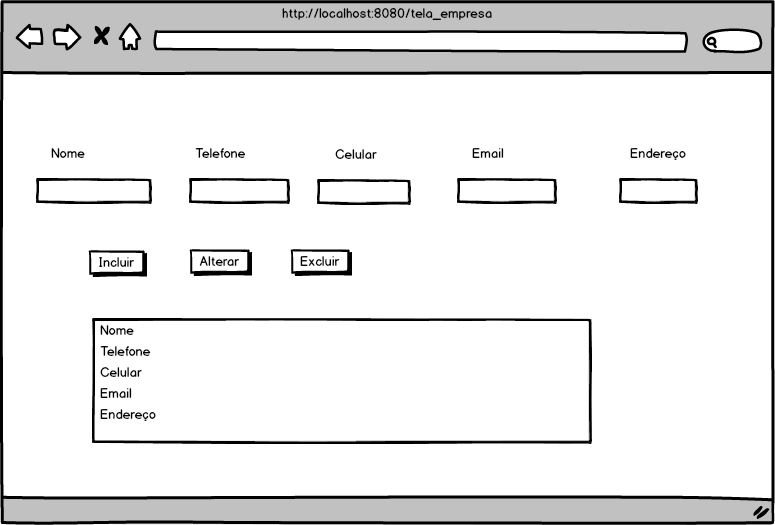
\includegraphics[scale=0.5]{imagens/prototipo_empresa.png}
 \caption{Protótipo - Tela de empresa.}
 \label{img:prototipo_empresa.png}
\end{figure}

A figura \ref{img:prototipo_empresa.png} demonstra a tela do sistema onde os
usuários poderam realizar um cadastro de um estágio.

\begin{figure}[!htb]
 \centering 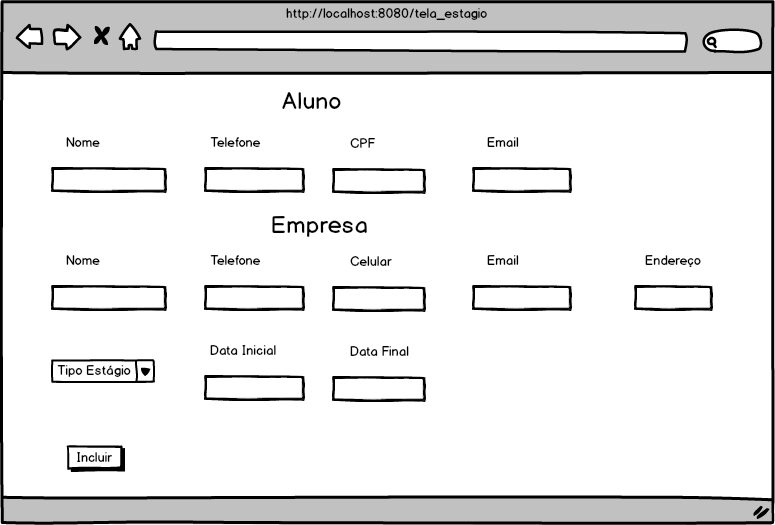
\includegraphics[scale=0.5]{imagens/prototipo_estagio.png}
 \caption{Protótipo - Tela de estágio.}
 \label{img:prototipo_estagio.png}
\end{figure}

A figura \ref{img:prototipo_orientacao.png} demonstra a tela do sistema onde os
usuários podem realizar um cadastro de orientação referente a um estágio.

\begin{figure}[!htb]
 \centering 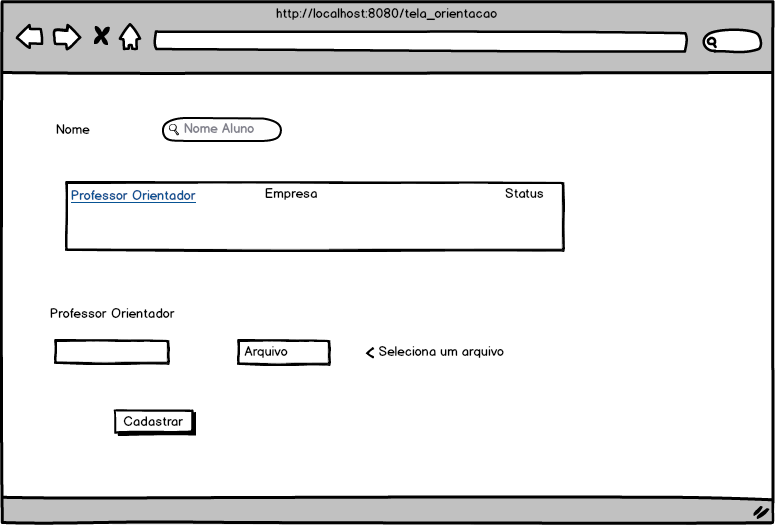
\includegraphics[scale=0.5]{imagens/prototipo_orientacao.png}
 \caption{Protótipo - Tela de orientação de estágio.}
 \label{img:prototipo_orientacao.png}
\end{figure}

A figura \ref{img:prototipo_colaboradorEmpresa.png} demonstra a tela do sistema
onde os usuários poderam realizar um C.R.U.D.

\begin{figure}[!htb]
 \centering 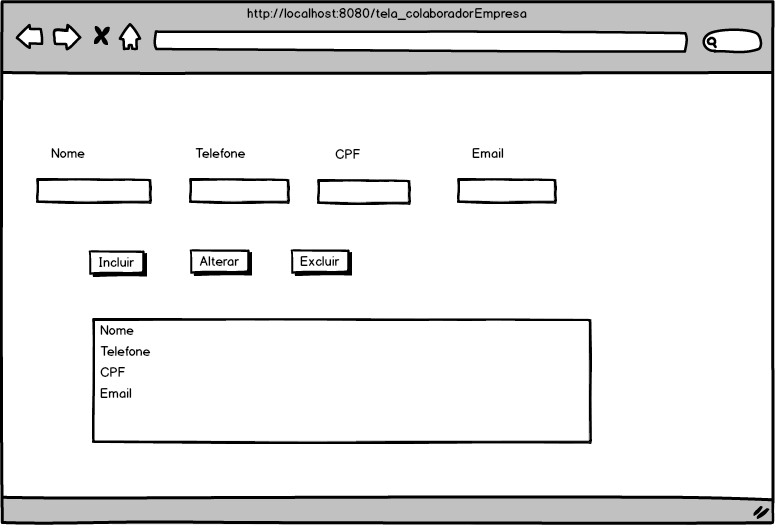
\includegraphics[scale=0.5]{imagens/prototipo_colaboradorEmpresa.png}
 \caption{Protótipo - Tela de colaborador da empresa.}
 \label{img:prototipo_colaboradorEmpresa.png}
\end{figure}

\section{Diagramas da UML}
\label{sec:diagramas}

A UML pode ser usada para visualizar, especificar, construir e documentar os
artefatos de um sistema de software-intensivo como descrito na Seção
\ref{subsec:uml}.

\subsection{Diagrama de Caso de Uso}
\label{sec:diagramaCasoUso}

Este documento serve para documentar o que o sistema faz do ponto de vista do
usuário, descrevendo as principais funcionalidades do sistema e a interação
dessas funcionalidades com os usuários do mesmo sistema.

A figura \ref{img:DiagramaDeCasoDeUso.png} demonstra
o Diagrama de Caso de Uso do sistema {\it SAGE}.

\begin{figure}[H]
 \centering 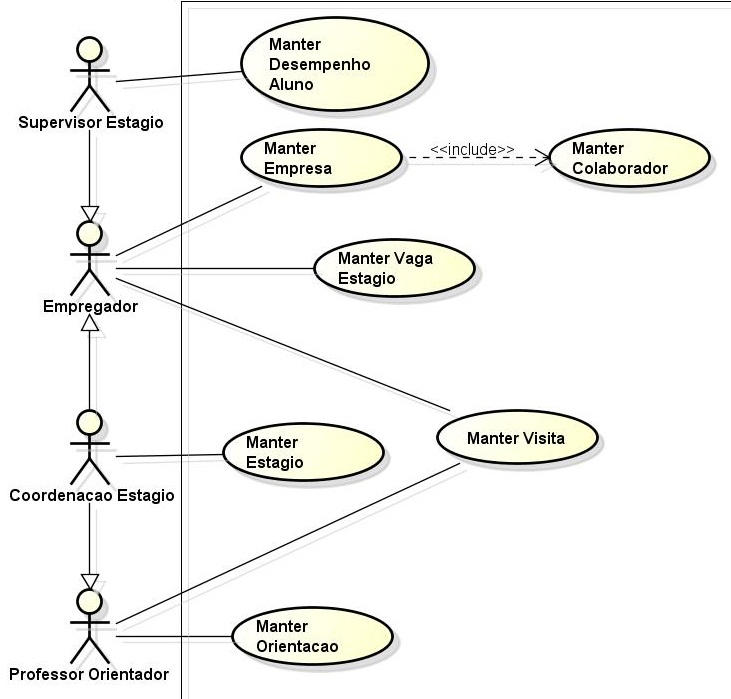
\includegraphics[scale=0.5]{imagens/DiagramaDeCasoDeUso.png}
 \caption{Diagrama de Caso de Uso.}
 \label{img:DiagramaDeCasoDeUso.png}
\end{figure}

\subsection{Diagrama de Atividade}
\label{sec:diagramaFluxo}

\subsection{Diagrama de Classe}
\label{sec:diagramaClasse}

A figura \ref{img:DiagramaDeClasse.png} demonstra o diagrama de classes UML do
sistema {\it SAGE}.

\begin{figure}[H]
 \centering 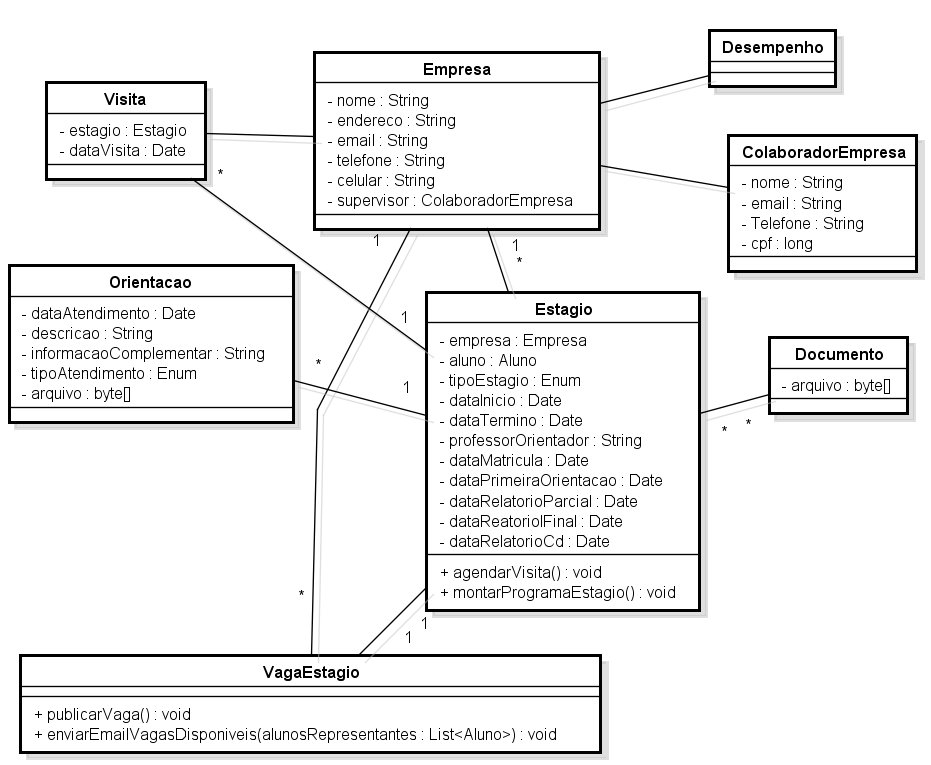
\includegraphics[scale=0.5]{imagens/DiagramaDeClasse.png}
 \caption{Diagrama de Classe UML - SAGE.}
 \label{img:DiagramaDeClasse.png}
\end{figure}

\section{Matriz de Rastreabilidade}
\label{sec:diagramas}

\section{Arquitetura do Software}
\label{sec:arquitetura}

\section{Frameworks e Ferramentas Adotadas}
\label{sec:frameworksFerramentasAdotadas}

\subsection{Astah Community}
\label{sec:astahcommunity}

Astah Community é um software para modelagem UML. É desenvolvido na plataforma
Java, o que garante sua portabilidade para qualquer plataforma que possui uma
máquina virtual Java. Foi utilizado para a modelagem UML por ser uma ferramenta
gratuita, e atender totalmente as necessidades do projeto ao desenvolver os
diagramas UML.

\subsection{Eclipse}
\label{sec:eclipse}

Eclipse é uma IDE gratuita open source feita em Java e atualmente a mais
utilizada no mundo. Um dos principais fatores que influenciaram o seu uso hoje
na versão (Kleper, 4.3.1) uso foi a sua enorme quantidade de plug-ins, que dão
um grande suporte aos desenvolvedores durante o desenvolvimento.

\subsection{Tomcat}
\label{sec:tomcat}

Tomcat é um servidor WEB Java, distribuído como software livre bastante
consolidado na comunidade, mantido pela Apache Software Fundation (Uma
organização sem fins lucrativos, que inclusive contribui ativamente com diversos
projetos para o Java). Esse servidor foi escolhido por ser um servidor gratuito
e de fácil instalação e por oferecer suporte a todos os recursos utilizados no
projeto.

\subsection{Java}
\label{sec:java}

A plataforma Java foi utilizada por hoje ser uma plataforma bastante consolidada
no mercado, um de seus grandes benefícios está em sua máquina virtual Java
(JVM), um grande conjunto de API e também a linguagem Java em si. Por ser uma
máquina virtual a JVM tem  importante característica nas aplicações feitas em
Java que é a portabilidade, outro recurso bastante interessante que a JVM nos
proporciona é a capacidade de executarmos outras linguagens já que a ela é
também multi-linguagem. Devido a sua popularização, o Java conta com um grande
apoio não só da comunidade como também de diversas empresas, o que resultou em
uma enorme variedade de ferramentas e bibliotecas o que a torna uma poderosa
ferramenta de desenvolvimento.

\subsection{Java Server Faces}
\label{sec:javaserverfaces}

O Java Server Faces (JSF) é uma especificação Java para arquitetura MVC, sua
arquitetura baseada em componentes o torna uma poderosa ferramenta para
construção de Ricas Interfaces com o Usuário (RIA), seu funcionamento orientado
a eventos faz com o que os desenvolvedores se dediquem menos em conhecer o
funcionamento do protocolo HTTP e dediquem-se mais na lógica da aplicação, o que
torna o seu funcionamento bem parecido com aplicações desktop. Sua arquitetura o
permite que desenvolvedores construam novos componentes baseado em componentes
já existentes, promovendo assim o reuso e a criação de componentes mais complexo.


\subsection{Primefaces}
\label{sec:primefaces}

Primefaces é uma poderosa biblioteca Java para a criação de Interfaces Gráficas
com o Usuário (GUI) para o JSF com uma série de componentes prontos. Este foi
utilizado devido ser hoje a mais recomendada no mercado, a frente de seus
concorrentes como RichFaces e IceFaces, e por ter o seu uso bastante simplificado.


\subsection{Spring}
\label{sec:spring}

Spring é um framework Java open source. Este foi utilizado visando realizar a
injeção de dependência e a inversão de controle, diminuindo o acoplamento entre
classes e melhorando a qualidade do código desenvolvido no projeto.


\subsection{Hibernate}
\label{sec:hibernate}

Hibernate é um software livre, open source para o mapeamento objeto-relacional
(ORM). Hoje ele é o ORM mais utilizado no mercado em aplicações Java. Ele foi
utilizado devido uma disparidade de paradigmas entre à programação orientada a
objetos e o banco de dados relacional, além de tirar do desenvolvedor o trabalho
de escreverem complexos scripts SQL, aumentando a produtividade da equipe. Um
recurso interessante disponibilizado por esta ferramenta é a possibilidade de
torna-lo independente de banco de dados, por realizar a intermediação entre a
aplicação e o banco de dados ele pode facilmente se adaptar a diversos bancos.


\subsection{Maven}
\label{sec:maven}

Apache Maven ou simplesmente Maven como é conhecido, é um projeto desenvolvido
pela Apache Software Foundation, essa ferramenta nos permite realizar a
construção, compilação e teste de aplicações Java de maneira simples e
automáticas. Essa ferramenta foi utilizada principalmente em nossos projetos por
ela realizar o gerenciamento das APIS de forma automatizada, padronizada,
facilitando e principalmente evitando problemas como conflitos de bibliotecas,
incompatibilidade de versões e a fácil localização de novas bibliotecas.


\subsection{Junit}
\label{sec:junit}

Junit é um framework open source para a realização de testes unitários em Java.
Ele facilita a criação de testes unitários como também a prática do TDD. Por ser
um framework bastante maduro e consolidado no mercado utilizando esse framework
por também se integrar ao Maven o que permite criar testes e automatiza-los,
esses testes seriam feitos sempre que realizarmos um deploy no projeto evitando
que falhas fossem disponibilizadas, mantendo a entrega de produtos mais confiável.
